\documentclass[english,floatsintext,man]{apa6}

\usepackage{amssymb,amsmath}
\usepackage{ifxetex,ifluatex}
\usepackage{fixltx2e} % provides \textsubscript
\ifnum 0\ifxetex 1\fi\ifluatex 1\fi=0 % if pdftex
  \usepackage[T1]{fontenc}
  \usepackage[utf8]{inputenc}
\else % if luatex or xelatex
  \ifxetex
    \usepackage{mathspec}
    \usepackage{xltxtra,xunicode}
  \else
    \usepackage{fontspec}
  \fi
  \defaultfontfeatures{Mapping=tex-text,Scale=MatchLowercase}
  \newcommand{\euro}{€}
\fi
% use upquote if available, for straight quotes in verbatim environments
\IfFileExists{upquote.sty}{\usepackage{upquote}}{}
% use microtype if available
\IfFileExists{microtype.sty}{\usepackage{microtype}}{}

% Table formatting
\usepackage{longtable, booktabs}
\usepackage{lscape}
% \usepackage[counterclockwise]{rotating}   % Landscape page setup for large tables
\usepackage{multirow}		% Table styling
\usepackage{tabularx}		% Control Column width
\usepackage[flushleft]{threeparttable}	% Allows for three part tables with a specified notes section
\usepackage{threeparttablex}            % Lets threeparttable work with longtable

% Create new environments so endfloat can handle them
% \newenvironment{ltable}
%   {\begin{landscape}\begin{center}\begin{threeparttable}}
%   {\end{threeparttable}\end{center}\end{landscape}}

\newenvironment{lltable}
  {\begin{landscape}\begin{center}\begin{ThreePartTable}}
  {\end{ThreePartTable}\end{center}\end{landscape}}




% The following enables adjusting longtable caption width to table width
% Solution found at http://golatex.de/longtable-mit-caption-so-breit-wie-die-tabelle-t15767.html
\makeatletter
\newcommand\LastLTentrywidth{1em}
\newlength\longtablewidth
\setlength{\longtablewidth}{1in}
\newcommand\getlongtablewidth{%
 \begingroup
  \ifcsname LT@\roman{LT@tables}\endcsname
  \global\longtablewidth=0pt
  \renewcommand\LT@entry[2]{\global\advance\longtablewidth by ##2\relax\gdef\LastLTentrywidth{##2}}%
  \@nameuse{LT@\roman{LT@tables}}%
  \fi
\endgroup}


  \usepackage{graphicx}
  \makeatletter
  \def\maxwidth{\ifdim\Gin@nat@width>\linewidth\linewidth\else\Gin@nat@width\fi}
  \def\maxheight{\ifdim\Gin@nat@height>\textheight\textheight\else\Gin@nat@height\fi}
  \makeatother
  % Scale images if necessary, so that they will not overflow the page
  % margins by default, and it is still possible to overwrite the defaults
  % using explicit options in \includegraphics[width, height, ...]{}
  \setkeys{Gin}{width=\maxwidth,height=\maxheight,keepaspectratio}
\ifxetex
  \usepackage[setpagesize=false, % page size defined by xetex
              unicode=false, % unicode breaks when used with xetex
              xetex]{hyperref}
\else
  \usepackage[unicode=true]{hyperref}
\fi
\hypersetup{breaklinks=true,
            pdfauthor={},
            pdftitle={A thorough evaluation of the Language Environment Analysis (LENATM) system},
            colorlinks=true,
            citecolor=blue,
            urlcolor=blue,
            linkcolor=black,
            pdfborder={0 0 0}}
\urlstyle{same}  % don't use monospace font for urls

\setlength{\parindent}{0pt}
%\setlength{\parskip}{0pt plus 0pt minus 0pt}

\setlength{\emergencystretch}{3em}  % prevent overfull lines

\ifxetex
  \usepackage{polyglossia}
  \setmainlanguage{}
\else
  \usepackage[english]{babel}
\fi

% Manuscript styling
\captionsetup{font=singlespacing,justification=justified}
\usepackage{csquotes}
\usepackage{upgreek}



\usepackage{tikz} % Variable definition to generate author note

% fix for \tightlist problem in pandoc 1.14
\providecommand{\tightlist}{%
  \setlength{\itemsep}{0pt}\setlength{\parskip}{0pt}}

% Essential manuscript parts
  \title{A thorough evaluation of the Language Environment Analysis
(LENA\textsuperscript{TM}) system}

  \shorttitle{LENA\textsuperscript{TM} evaluation}


  \author{many\textsuperscript{1}}

  % \def\affdep{{""}}%
  % \def\affcity{{""}}%

  \affiliation{
    \vspace{0.5cm}
          \textsuperscript{1}   }

  \authornote{
    Correspondence concerning this article should be addressed to many, .
    E-mail:
  }


  \abstract{In the previous decade, dozens of studies involving thousands of
children across several research disciplines have made use of a combined
daylong audio-recorder and automated algorithmic analysis called the
LENA\textsuperscript{TM} system, which aims to assess children's
language environment. While the system's prevalence in the language
acquisition domain is steadily growing, there are only scattered
validation efforts, on only some of its key characteristics. Here, we
assess the LENA\textsuperscript{TM} system's accuracy across all of its
key measures: speaker classification, adult word counts (AWC), child
vocalization counts (CVC), and conversational turn counts (CTC). Our
assessment is based on manual annotation of clips that have been
randomly or periodically sampled out of daylong recordings, collected
from (a) populations similar to LENA\textsuperscript{TM}`s original
training data (North American English-learning children aged 3-36
months), (b) children learning another dialect of English (UK), and (c)
slightly older children growing up in a different linguistic and
socio-cultural setting (Tsimane' learners in rural Bolivia). We find
reasonably high accuracy in some measures (AWC, CTC), with more
problematic levels of performance in others (CTC, precision and recall
of male adults and other children). We find little difference in
accuracy as a function of child age, dialect, or socio-cultural setting.
Whether LENA\textsuperscript{TM} results are accurate enough for a given
research, educational, or clinical application depends largely on the
specifics at hand. We therefore conclude with a set of recommendations
to help researchers make this determination for their goals.}
  



  \usepackage{array}
  \usepackage{float}

\begin{document}

\maketitle

\setcounter{secnumdepth}{0}



While nearly all humans eventually become competent users of their
language(s), documenting the experiential context of early acquisition
is crucial for both theoretical and applied reasons. Regarding theory,
there are many open questions about what kinds of experiences and
interactions are necessary, sufficient, or optimal for supporting
language development. Moreover, the ability to accurately and quickly
assess an infant's state of development at a given point in time is of
central importance for clinical purposes, both for children with known
risks of language delays and disorders, and those who might not be
identified based on risk factors. Reliable assessments are also crucial
for measuring intervention efficacy.

One approach that has been making its way into the mainstream literature
across basic and applied research on language and cognition relies on
day-long recordings gathered with a LENA\textsuperscript{TM}
audiorecorder (J. Gilkerson et al., 2017; e.g., Greenwood,
Thiemann-Bourque, Walker, Buzhardt, \& Gilkerson, 2011; Oller et al.,
2010), and further analyzed using LENA\textsuperscript{TM}'s automated,
closed-source algorithms. As we summarize below, this approach has many
advantages, which may explain its expanding popularity. While dozens of
papers over the past decade have used LENA\textsuperscript{TM}'s
automated output, only a handful include validity estimates (d'Apice,
Latham, \& Stumm, 2019; e.g., Weisleder \& Fernald, 2013; Zimmerman et
al., 2009), even fewer where validity estimation was the primary focus
of the paper (F. Bulgarelli \& Bergelson, in press; e.g., Canault, Le
Normand, Foudil, Loundon, \& Thai-Van, 2016; Ganek \& Eriks-Brophy,
2018; Lehet, Arjmandi, Dilley, Roy, \& Houston, 2018). As a result, few
studies report sufficient details about validation accuracy for one or
more metrics, limiting the interpretability of the results of a
meta-analytic assessment (as attempted in A. Cristia, Bulgarelli, \&
Bergelson, 2019).

The work undertaken thus far also has some limitations, which are
described further in the \enquote{Previous Validation} section below,
and mentioned briefly next. First, many validations or evaluations of
LENA\textsuperscript{TM} omit analysis of the less-directly
\enquote{relevant} categories of input like noise, silence, or overlap.
Second, many LENA\textsuperscript{TM} evaluations rely on
LENA\textsuperscript{TM}\enquote{s own output as a starting point to
either select portions of the file for manual annotation, or use its
segmentation into talker turns or vocalizations as the unit of analysis
rather than segmenting the audio from scratch. Both decisions can lead
to inflated accuracy estimates. Here we endeavor to conduct an
evaluation that is fully independent of the LENA\textsuperscript{TM}
algorithms} automated assessment, permitting a systematic, extensive,
and independent evaluation of its key metrics.

In a nutshell, this paper reports on the performance of
LENA\textsuperscript{TM} algorithms when compared to human annotations
carried out in a clips extracted from daylong audiorecordings gathered
from (a) a sample of children similar to the LENA\textsuperscript{TM}
training set (i.e.~infants and toddlers, growing up in North American
English-speaking homes, and aged 3-36 months), (b) a group of similarly
aged children learning a different dialect (UK English); and (c)
slightly older children learning a different language in a very
different sociocultural setting (Tsimane'-learning children in rural
Bolivia).

\subsubsection{\texorpdfstring{Brief introduction to
LENA\textsuperscript{TM}
products}{Brief introduction to LENATM products}}\label{brief-introduction-to-lenatm-products}

The LENA\textsuperscript{TM} system consists of a hardware component (a
lightweight, sturdy, and easy-to-use recording device worn by a child in
specialized clothing) and a suite of proprietary computer programs
designed to provide automated quantitative analyses of the auditory
environment and the child's own vocalizations. The latter was developed
over an extensive corpus of full day audio recordings gathered using
their patented recording hardware (Xu, Yapanel, \& Gray, 2009). The
original dataset included over 65,000 hours of recording across 329
American English-speaking families chosen for diversity in child age
(1-42 months) and socio-economic status (J. Gilkerson \& Richards,
2008). Half-hour selections from 309 recordings were transcribed and
annotated for the purpose of developing the algorithm, and an additional
60 minutes from each of 70 recordings were transcribed and annotated for
testing the result (Gilkerson, Coulter, \& Richards, 2008).

The resulting LENA\textsuperscript{TM} software takes as input a new
audio recording and processes it incrementally in short windows,
extracting a variety of acoustic features which are used to classify the
audio stream into segments of at least 600 ms in length (or longer for
some of the categories) using a Minimum Duration Gaussian Mixture Model
(MDGMM; Xu et al., 2009). Silence may be included to \enquote{pad}
segments to this minimum duration. The segments are classified according
to a set of broad speaker and non-speaker classes. The speaker classes
are: Male Adult, Female Adult, \enquote{Key} Child (i.e.~the one wearing
the recorder) and Other Child. The non-speaker classes are: Noise,
Television (including any electronics), Overlap (speech overlapped with
other speech or nonspeech sounds), and Silence (SIL). With the exception
of Silence, these classifications are then passed through a further
likelihood test between the original classification for a given segment
and the Silence class, the result of which determines whether they are
\enquote{Near} (high probability of being that class) or \enquote{Far}
(low probability, they may be silence instead). Given the large number
of acronyms and labels of various kinds, we provide a listing of
relevant LENA\textsuperscript{TM} abbreviations on Table 1; in what
follows, we highlight the specific labels that we evaluate in the
present work in bold.

After this broad speaker classification step, Female or Male Adult
\enquote{Near} segments (FAN and MAN) are further processed using an
adaptation of the Sphinx Phone Decoder (Lamere et al., 2003) in order to
form an automated estimate of the number of words in each segment (Adult
Word Count, or \textbf{AWC}). Key Child (CHN) segments are further
processed to sub-classify regions in them into vegetative noises,
crying, and speech-like vocalizations. LENA\textsuperscript{TM} provides
the count (child vocalization count, or CVC) and duration of the latter,
speech-like sub-segments. A further metric, Conversational Turn Counts
(CTC), reflects the number of alternations between an adult and the key
child (or vice versa), bounded by maximally 5 s of non-speech.

\begin{table}[t]

\caption{\label{tab:tab-abb}A partial listing of common LENA abbreviations and their meanings.}
\centering
\begin{tabular}{>{\raggedright\arraybackslash}p{10em}>{\raggedright\arraybackslash}p{30em}}
\toprule
Abbreviations & Meanings\\
\midrule
FAN, MAN, CHN, CXN & Basic “meaningful speech” (near and clear speech) categories used by LENA for further processing: Female Adult Near, Male Adult Near, Key Child Near and Other Child Near categories respectively.\\
NON, TVN, OLN, SIL & Basic non-speech categories: Noise Near,  Television Near, Overlap Near, Silence.\\
FAF, MAF, etc. & “Far” (low probability) versions of each category.\\
Key child & Child wearing recorder\\
AWC & Adult Word Count (estimated within FAN and MAN vocalizations)\\
\addlinespace
AVA & A measure of vocal maturity processed over VOC\\
CVC & Child Vocalization Count (estimated for non-cry, non-vegetative portions of CHN)\\
CTC & Conversational Turn Count (estimated over FAN/MAN and CHN turns)\\
\bottomrule
\end{tabular}
\end{table}

\subsubsection{Previous validation work}\label{previous-validation-work}

A recent systematic review (A. Cristia et al., 2019) found 23 papers,
containing 28 studies, reporting on the accuracy of
LENA\textsuperscript{TM}\enquote{s labels and derived metrics (AWC, CVC,
CTC). They conclude that there are \enquote{reasonably good results
{[}overall{]}: over 61\% for recall and precision based on 11-12
non-independent studies; correlations for AWC mean r=.79, on n=11, with
a mean RER {[}i.e., Relative Error Rate{]}=10\% on n=11; CVC mean r=.76,
n=5, with a mean RER=1\% on n=5. The exception to this general trend
towards good performance was CTC, with a mean r=.31, n=5, RER=-64\% on
n=2.} The systematic review also identified several limitations of the
body of previous validation work. First, for the majority of included
studies, the validity report was not fully evaluated by peer review.
Even if the study may have appeared in a journal with a peer reviewed
process, the validation in itself was often a secondary goal to support
a different research objective, and therefore often lacked
methodological details or even full results. For instance, Seidl et al.
(2018) report on validation of LENA\textsuperscript{TM} labels among
children at familial risk for autism in a one-paragraph appendix to the
paper, which only mentions confusions between female adult and child. It
is not clear whether confusions between key child and any other category
(other child, male adult, silence, etc.) were ignored rather than
counted as an error. While this approach may be reasonable for a given
study's research goals, it has the undesirable side effect of creating
the impression that LENA\textsuperscript{TM} metrics are widely
validated, while in fact validation methods may not have been reported
or evaluated in detail. Second, previous studies typically did not take
silence, noise, or overlap into account in the reported confusion
matrices or other accuracy measures, particularly within segments. That
is, if a LENA\textsuperscript{TM} segment labeled \enquote{key child}
contained one second of silence and two seconds of speech by the key
child, the full three second clip may be tagged as 'correct} though it
was only 67\% correct, leading to an overestimation of the accuracy of
the \enquote{key child} label.

Third, a majority of previous validation studies used the
LENA\textsuperscript{TM} output itself to select the sections that would
be annotated for validation (in A. Cristia et al., 2019, this held for
14/25 studies that specified the method of selection). For instance,
clips may have been selected for manual annotation on the basis of high
AWC and/or CTC according to the algorithm. This unfortunately leads to
biased sampling: Since LENA\textsuperscript{TM} only counts words within
FAN and MAN segments and conversational turns involving FAN/MAN
alternations with CHN in close proximity, high AWC or CTC can only occur
in sections of the recording that are \enquote{clean} enough for the
algorithm to parse; otherwise, most of the section would have been
classified as overlap (OLN), which does not count towards AWC or CTC.
This would tend to bias these reports toward a higher level of accuracy
than would be obtained across the full recording.

Forth, previous validation work has typically focused on a single
corpus, participant population, age range, and language. As a result,
although considerable variation in performance has sometimes been
reported (Canault et al., 2016; e.g., J. Gilkerson et al., 2016) it is
difficult to assess whether a numerical difference in accuracy found is
significant, and if so, whether this is due to a difference in the way
the corpus was constituted and annotated, rather than on how
LENA\textsuperscript{TM} fares with that population, age range, and
language.

\subsubsection{The present work}\label{the-present-work}

We sought to assess the validity of LENA\textsuperscript{TM}'s metrics
through an approach that complements the preceding literature.
Specifically, we report an evaluation of all speech labels and some
non-speech labels of LENA\textsuperscript{TM}, namely: silence (SIL),
overlap near (OLN), overlap far (OLF); as well as
LENA\textsuperscript{TM}'s key derived metrics: adult word count (AWC),
conversational turn count (CTC), and child vocalization count (CVC). We
aim to address several of the limitations found in the body of previous
work.

First, to maximally avoid potential bias in our annotations, we used
random or periodic sampling (detailed below) to choose which sections of
daylong recordings to annotate, and did not give annotators access to
the LENA\textsuperscript{TM} output. Second, to allow assessment of the
accuracy of the segmentation itself as well as categorical labeling,
evaluation is done at the level of 10 ms frames rather than segments.
This allows us to capture a much finer-grained representation of the
auditory environment (i.e., if LENA\textsuperscript{TM} classified a 2 s
audio segment as FAN, but .8 s of this was actually non-speech noise or
a different talker, LENA\textsuperscript{TM} would be credited only for
the proportion that was correct).

Third, to gain traction on generalizability, rather than focusing on a
single sample that either mirrors or diverges from
LENA\textsuperscript{TM}s original population, we included five corpora.
Three corpora sampled from the same population, language, dialect, and
age group the LENA\textsuperscript{TM} softawer was developed with. A
fourth corpus was chosen to allow an extension to a different dialect of
English. The fifth corpus constituted an extension to a totally
different recording condition (a rural setting, with large families and
many children present, in a typologically different language). The age
range also varies a great deal, and it is slightly higher in this last
corpus.

Finally, the present study relies on a collaborative annotation effort
across several labs. Critically, this means that we can \enquote{fairly}
compare annotations across our corpora: annotation decisions were either
identical or conceptually comparable, and all analyses were identical.
This allows us to more readily answer questions regarding differences in
reliability as a function of e.g.~child age and language. Also, by
looking at corpora that were not annotated in exactly the same way, we
can better infer the likelihood with which our results will generalize
to other corpora, even if they are not annotated exactly in the same
way.

\subsection{Methods}\label{methods}

\subsubsection{Corpora}\label{corpora}

The data for the evaluation comes from five different corpora, annotated
in the context of two research projects. The largest one is the ACLEW
project (Bergelson et al., 2017; Soderstrom et al., in progress); in
this paper we focus on four different corpora of child daylong
recordings that have been pooled together, sampled, and annotated in a
coordinated manner. These four corpora are: the Bergelson corpus
(\enquote{BER}) from US English families from the upstate New York area
(Bergelson, 2016), the LuCiD Language 0--5 corpus (\enquote{L05})
consisting of English-speaking families from Northwest England (C. F.
Rowland, Bidgood, Durrant, Peter, \& Pine, 2018), the McDivitt and
Winnipeg corpora (\enquote{MCD}) of Canadian English families (McDivitt
\& Soderstrom, 2016), and the Warlaumont corpus (\enquote{WAR}) of US
English from Merced, California (A. Warlaumont, Pretzer, Walle, Mendoza,
\& Lopez, 2016). Some recordings in BER, and all recordings in MCD and
WAR are available from HomeBank repository (VanDam et al., 2016). The
second project contains a single corpus collected from Tsimane' speaking
families in Bolivia (``TSI''; C. Scaff, Stieglitz, Casillas, \& Cristia,
in progress). Socioeconomic status varies both within and across
corpora. Key properties of the five corpora are summarized in Table 2.

\begin{table}[t]

\caption{\label{tab:tab-corp}Key properties of the five corpora}
\centering
\begin{tabular}{>{\centering\arraybackslash}p{1cm}>{\centering\arraybackslash}p{2.5cm}>{\centering\arraybackslash}p{1.5cm}>{\centering\arraybackslash}p{3cm}>{\centering\arraybackslash}p{3.5cm}>{\centering\arraybackslash}p{3.5cm}}
\toprule
Corpus & Children & Clips & Clip dur 
 (in seconds) & Age mean (range) in months & Location\\
\midrule
WAR & 10 & 150 & 120 & 6.3 (3-9) & Western US\\
BER & 10 & 150 & 120 & 11.2 (7-17) & Northeast US\\
SOD & 9 & 150 & 120 & 12.3 (2-32) & Western Canada\\
L05 & 10 & 150 & 120 & 20 (11-31) & Northwest England\\
TSI & 10 & 272 & 60 & 34 (15-58) & Northern Bolivia\\
\bottomrule
\end{tabular}
\end{table}

Despite these differences, all five corpora consists of long (4--16
hour) recordings collected as children wear a LENA\textsuperscript{TM}
recorder in a LENA\textsuperscript{TM} vest throughout a normal day
and/or night. For the four ACLEW corpora, out of the 106 recorded
participants, daylong recordings from 10 infants from each corpus were
chosen for manual annotation, selected to represent a diversity of ages
(0--36 months) and socio-economic contexts. In the SOD corpus, sensitive
information was found in one of the files, and thus one child needed to
be excluded. The tenth day for this corpus was a second day by one of
the 9 included children. From each daylong file, fifteen 2-minute
non-overlapping audio (with a 5-minute context window) were randomly
sampled from the entire daylong timeline for manual annotation. This
30-minute sample corresponded to approximately 1 minute of annotated
speech per key child (collapsing across all speaker categories).

The TSI corpus consisted of 1 or 2 recordings from 12 children, out of
the 25 children recorded from field work that year; the other 13 had
been recorded using other devices (not the LENA\textsuperscript{TM}
hardware). From these files, 1-minute segments were sampled in a
periodic fashion. That is, for each recording, we skipped the first 33
minutes to allow the family to acclimate to the recorder, and then
extracted 1 minute (with a 5-minute context window) every 60 minutes,
until the end of the recording was reached. This resulted in 4 to 16
minutes of manually annotated audio per child per recording (mean =
12.64 minutes), and an average of 3 minutes of speech per key child
(collapsing across all speaker categories).

We chose to sample 1 or 2 minutes at a time (TSI, and ACLEW corpora,
respectively) because conversations are likely to be bursty (Goh \&
Barabási, 2008). That is, it is likely the case that speech is not
produced at a periodic rate (e.g., one phrase every 20 seconds), but
rather it occurs in bursts (a conversation is followed by a long period
of silence between the conversational partners, followed by another bout
of conversation, perhaps with different interlocutors, followed by
silence, and so on). In this context, imagine that you sample a 5-second
stretch. If you find speech in that stretch, then it is likely you have
by chance fallen on a conversation bout; if you do not find speech, then
you have likely found a silence bout. If you were to extend that
selection out to several minutes, then it is likely that you will simply
add more material from the same type (i.e.~conversation bout or silence
bout). As a result, any sampling method that favors medium-sized
stretches (5-15 minutes) will tend to end up with samples that are
internally homogeneous (throughout the 5 minutes, there is a
conversation), but highly heterogeneous as a collection if sampling is
random throughout the day. This in turn would lead to artificially high
correlations between LENA\textsuperscript{TM} and human metrics in all
dependent variables (e.g., since probably little speech, fewer turns,
and fewer child vocalizations will be found in silent bouts and more in
conversational ones). Thus, our strategy of sampling
randomly/periodically and in short stretches is more likely to capture
finer-grained variation in speech quantity.

In the 5 corpora, the 1- or 2-min samples were annotated for all
hearable utterance boundaries and talker ID. In ACLEW corpora
\footnote{see @casillas2017a and  @casillas2017b for the general annotation protocol, and @soderstrom, for an introduction to the databases.},
talker IDs reflected unique individual talkers, but were coded in such a
way to readily allow mapping onto LENA\textsuperscript{TM}s talker
categories (e.g.~key child, other child 1, female adult 1, female adult
2). In the TSI corpus, only the key child and one female adult whose
voice recurred throughout the day were individually identified, with all
other talkers being classified on the basis of broad age and sex into
male adult, female adult, and other children. The ACLEW datasets had
other coding levels which will not be discussed here.

\subsubsection{Processing}\label{processing}

Several different time units are needed to clarify how each metric is
calculated (see Figure 1). Clips refer to the 1- or 2-minute samples
extracted from recordings. This is the basic unit at which child
vocalization counts and conversational turn counts can be established.
In addition, since most previous work evaluating adult word counts did
so at the clip level, we do so here as well.

\begin{figure}
\centering
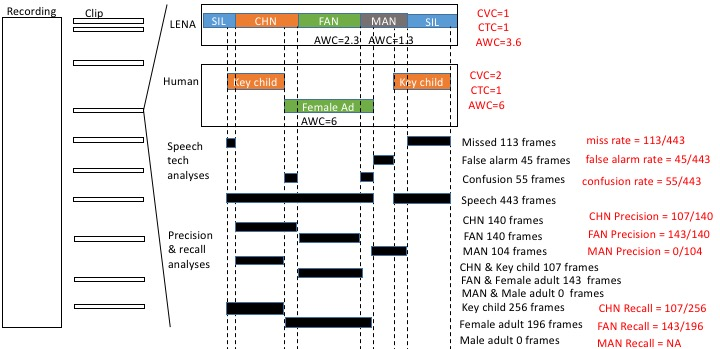
\includegraphics{fig_levels.jpg}
\caption{Levels at which performance is evaluated.}
\end{figure}

The other metrics require a more detailed explanation, conveyed
graphically in Figure 1. The stretch of time that has been assigned to a
speech or non-speech class by LENA\textsuperscript{TM} is a
\emph{segment}. In one clip, there may be just one long segment (e.g.,
the whole clip has been assigned to Silence by
LENA\textsuperscript{TM}); or there may be more (e.g., the first 5
seconds are attributed to the key child, then there is a 50-second
Silence segment, and the final 5 seconds are attributed to a Female
Adult). In LENA\textsuperscript{TM}'s automated analysis, only one of
these categories may be active at a given point in time. In contrast, we
typically speak of utterances or vocalizations to refer to stretches of
speech detected by humans and assigned to different talkers. Again,
clips may have zero or more utterances. Unlike LENA\textsuperscript{TM},
however, a given point in time may be associated with multiple speakers.
Given that there need not be a one-to-one correspondence between
LENA\textsuperscript{TM} segments and human utterances, we need to
define smaller time units that can be used to check for agreement. In
this paper, we use 10 ms frames. This is the basic time unit used for
all classification accuracy estimations, which are introduced in more
detail in the next subsection.

\subsubsection{\texorpdfstring{LENA\textsuperscript{TM} classification
accuracy}{LENATM classification accuracy}}\label{lenatm-classification-accuracy}

Our first goal was to establish LENA\textsuperscript{TM} talker tag
accuracy, particularly for the four broad LENA\textsuperscript{TM}
talker categories (key child, other child, female adult, male adult; or
CHN, CXN, FAN, MAN), but taking into account other categories (with some
limitation on their interpretation). We calculated accuracy in two
complementary ways. First, we used three frame-based standard metrics of
speech and talker segmentation to allow direct comparison with other
systems in the speech technology literature (False Alarm Rate, Miss
Rate, Confusion Rate). We also use Diarization Error Rate, which is
derived by summing the first three metrics; together these provide a
stringent and standard test of accuracy. Second, we used frame-based
precision and recall of each category to provide an intuitive
representation of the error patterns shown by this system.

\paragraph{Speech and talker segmentation
metrics}\label{speech-and-talker-segmentation-metrics}

The original coding was converted using custom-written python scripts
into a standard adaptation of the \enquote{Rich Transcription Time Mark}
(rttm) format (Ryant et al., 2019), which indicates, for each
vocalization or segment, its start time, duration, and speaker. This
representation was used in pyannote.metrics (Bredin, 2017) to compute
four standard diarization metrics: rate of false alarm for speech, rate
of misses for speech, rate of confusion between talkers, and the derived
diarization error rate (DER). These are calculated with the following
formulas at the level of each clip, where FA (false alarm) is the number
of frames during which there is no talk according to the human annotator
but during which LENA\textsuperscript{TM} found some talk; M (miss) is
the number of frames during which there is talk according to the human
annotator but during which LENA\textsuperscript{TM} found no talk; C
(confusion) is the number of frames correctly classified as
LENA\textsuperscript{TM} as containing talk, but whose voice type has
not been correctly identified (when the LENA\textsuperscript{TM} model
recognizes female adult speech where there is male adult speech for
instance), and T is the total number of frames that contain talk
according to the human annotation:

\begin{itemize}
\tightlist
\item
  false alarm rate = FA/T,
\item
  miss rate = M/T,
\item
  confusion rate = C/T,
\item
  DER = (FA+M+C)/T,
\end{itemize}

In the human annotation, there is no class representing overlapping
speech as such. For the sake of completeness and full comparison with
the LENA\textsuperscript{TM} model, if two or more different speech
sources were active at the same time according to the human annotators,
these frames have been mapped to the class \enquote{overlap} post hoc.
This allows us to compare this Overlap class to
LENA\textsuperscript{TM}'s OLN (and, for the precision/recall analysis
introduced next, OLF) by the LENA\textsuperscript{TM} model. Therefore,
in the most complete analysis, the confusion rate is computed based on
the human-LENA\textsuperscript{TM} matches in Table 3.

\begin{table}[t]

\caption{\label{tab:tab-tsicor}Correspondances between LENA and our human annotation. Additional analyses remove one or both of the last two rows. *Electronic voices were only annotated in the ACLEW dataset. Although some Tsimane' families listen to the radio, radio speech was not annotated in the TSI corpus.}
\centering
\begin{tabular}{>{\raggedright\arraybackslash}p{2cm}>{\raggedright\arraybackslash}p{2cm}}
\toprule
LENA & Human\\
\midrule
CHN & CHI\\
CXN & OCH\\
FAN & FA\\
MAN & MA\\
TVN* & E*\\
\addlinespace
OLN & OL\\
\bottomrule
\end{tabular}
\end{table}

However, the overlap category is not defined the same way as the
LENA\textsuperscript{TM} overlap category. For LENA\textsuperscript{TM},
overlap between any two categories is labeled OLN -- i.e., Noise + TV
would be counted towards overlap as would FAN+FAN; whereas for us, only
overlap between two talker categories (e.g., key child and female adult,
noise was not coded) counts as overlap. Similarly, the TVN
LENA\textsuperscript{TM} class is not equivalent to the electronic
speech tag in the ACLEW coding, because the former also includes music,
singing, crowd noise and any other sound coming from a TV or another
electronic source, whereas the latter only includes speech from an
electronic source. Therefore, additional analyses map these classes onto
\enquote{silence} post hoc, so as to not penalize confusions involving
them.

\paragraph{Precision and recall}\label{precision-and-recall}

This evaluation looks in more detail at the pattern of errors, by
assessing how LENA\textsuperscript{TM} and human annotators agreed and
disagreed. In both precision and recall, the numerator is the
intersection between a LENA\textsuperscript{TM} tag and a human tag
(e.g., the number of frames that LENA\textsuperscript{TM} classified as
CHN and the annotator classified as Key child; notice, there is no
constraint that these two categories by conceptually the same). The
denominator differs: To calculate precision, we divide that number by
the total number of frames attributed to a category by
LENA\textsuperscript{TM}, whereas for recall, we divide by the total
number of frames attributed to a category by the human annotator.

\subsubsection{CVC and CTC evaluation}\label{cvc-and-ctc-evaluation}

From the human annotation, each vocalization by the key child counted
towards the total Child Vocalization Count (CVC) for a given clip. For
the Conversational Turn Count (CTC), a sequence of key child and any
adult (or vice versa) within 5 seconds counted towards the clip total
CTC. The Pearson correlation across LENA\textsuperscript{TM} and human
estimations were calculated.

Users may also wish to interpret the absolute number of vocalizations or
turns found by LENA\textsuperscript{TM}. Therefore, it is important to
also bear in mind absolute error rates, relative error rates, and
relative absolute error rates. Despite the similarity in their names,
these three metrics provide different information. The absolute error
rate tells us, given a LENA\textsuperscript{TM} estimate, how close the
actual number may be, as it is calculated as NL-NH, where NL the number
according to LENA\textsuperscript{TM} and NH is the number according to
humans. By averaging across clips, we then get an idea of the bias
towards overestimation (if this number is positive) or underestimation
(if this difference is negative).

The relative error rate puts this bias in relation to the actual number
of vocalizations tagged by the human coder: (NL-NH)/NL. For instance,
imagine that we find that LENA\textsuperscript{TM} errs by 10
vocalizations on average according to the average absolute error rate;
this means that, on average across short clips like the ones used here,
the numbers by LENA\textsuperscript{TM} would be off by 10
vocalizations. We may think this number is small; by using the relative
error rate, we can check whether it is small relative to the actual
number found: An error of 10 vocalizations would seem less problematic
if there are 100 vocalizations on average (LENA\textsuperscript{TM}
would be just 10\% off) than if there are 10 (LENA\textsuperscript{TM}
would be doubling the number of vocalizations). As with the absolute
error rate, the sign of this difference indicates whether
LENA\textsuperscript{TM} tends to over- or under-estimate these counts.

Finally, the relative absolute error rate is calculated with the formula
abs(NL-NH)/NL, where abs indicates that one takes the absolute of the
difference. As a result, it cannot be used to assess systematic under-
or over-estimation biases, but rather gives an idea of how accurate the
estimates are at the clip level (statistically speaking). To convey this
intuitively, one could find absolute error rates and relative error
rates that are 0 because Otherwise the estimates could be half -100
vocalizations off (for absolute error rates) or -100\% off (for the
relative error rates), with the other half behaving in the exact
opposite fashion.

\subsubsection{AWC evaluation}\label{awc-evaluation}

For the AWC portion of this evaluation, we could only use transcriptions
from the four ACLEW corpora, since the TSI corpus has not been
transcribed (and thus lacks word counts). Annotators for the four ACLEW
corpora were proficient in the language spoken in the daylong recording,
and transcribed all adult speech based using canonical lexical forms
(e.g. \enquote{wanna}, not \enquote{want to}) in keeping with minCHAT
format (MacWhinney, 2017).

Reference adult word counts were determined by counting all
unambiguously transcribed words spoken by adult talkers. This was
achieved by first discarding all non-lexical transcript entries such as
non-linguistic communicative sounds, paralinguistic markers, and markers
indicating incomprehensible speech. In addition, all utterances from the
key child and other children were omitted from the Adult Word Count. The
remaining orthographic entries separated by whitespaces were then
counted as gold standard target words for LENA\textsuperscript{TM} to
detect. One child in the SOD corpus was learning French. Given our
definition of orthographic words with no language-specific processing,
we have included this child to increase power, but results without them
are nearly identical.

As for LENA\textsuperscript{TM} word counts, the regions sampled for
manual annotation were not guaranteed to perfectly align with
LENA\textsuperscript{TM} segments, and human utterances need not align
with them either. Of all LENA\textsuperscript{TM} segments overlapping
with human vocalizations, 14\% had only partial overlap with the
annotations. To match LENA\textsuperscript{TM} AWCs with the annotated
word counts, words from the partially overlapping
LENA\textsuperscript{TM} utterances were included in proportion to the
amount of overlap between the LENA\textsuperscript{TM} turn and the
reference segment in question (e.g., if 10\% of a
LENA\textsuperscript{TM} segment overlapped with a manually-annotated
utterance, 10\% of the total LENA\textsuperscript{TM} AWC estimate for
that segment was included in the LENA\textsuperscript{TM} word count
estimate for that utterance).

AWC were evaluated using Pearson correlations and error rates, similarly
to CVC and CTC.

\subsection{Results}\label{results}

Before starting, we provide some general observations based on the human
annotation. Silence is extremely common, constituting 79\% of the
frames. In fact, 45\% of clips contained no speech by any of the speaker
types (according to the human annotators). As for speakers, female
adults make up 11\% of the frames, the child contributes to 4\% of the
frames, whereas male adult voices, other child voices, and electronic
voices are found in only 1\% of the frames each. Overlap makes up the
remaining 3\% of the frames. The following consequences ensue. If
frame-based accuracy is sought, a system that classifies every frame as
silence would be 79\% correct. This is of course not what we want, but
it indicates that systems well adapted to this kind of speech should
tend to have low false alarm rates, being very conservative as to when
there is speech. If the system does say there is speech, then it had
better say that this speech comes from female adults, who provide a
great majority of the speech, nearly 3 times as much as the key child
and 10 times more than other children or male adults. In fact, given
that speech by male adults and other children is so rare, a system that
makes a lot of mistakes in these categories may still have a good global
performance, because these categories jointly account for only 2\% of
the frames.

\subsubsection{\texorpdfstring{LENA\textsuperscript{TM} classification
accuracy: False alarms, misses,
confusion}{LENATM classification accuracy: False alarms, misses, confusion}}\label{lenatm-classification-accuracy-false-alarms-misses-confusion}

Our first analysis is based on standard speech technology metrics, which
put errors in the perspective of how much speech there is. That is, if
10 frames are wrong in a file where there are 100 frames with speech,
this is a much smaller problem than if 10 frames are wrong in a file
where there is 1 frame with speech. In other words, these metrics should
be considered relative error metrics. One problem, however, emerges when
there is no speech whatsoever in a given file. In the speech technology
literature, this is never discussed, because most researchers working on
this are basing their analyses on files that have been selected to
contain speech (e.g., recorded in a meeting, or during a phone
conversation). We still wanted to take into account clips with no speech
inside because it is key for our research goals: We need systems that
can deal well with long stretches of silence, because we want to measure
in an unbiased manner how much speech children hear. Unfortunately, in
the 45\% of clips that had no speech whatsoever, the false alarm, miss,
and confusion rates are all undefined, because the denominator is zero.
In all likelihood, this leads to an overestimation of
LENA\textsuperscript{TM}'s performance, because potential false alarms
in these files are not counted against the system. It also occurred that
there was just a little speech; in this case, the denominator is very
small, and therefore the ratio for these two metrics ended up being a
very large number. Since means are not robust to outliers, we report on
medians.

As mentioned briefly above, there were, a priori, several ways of
analyzing the data:

\begin{itemize}
\tightlist
\item
  collapsing near and far together (i.e., CHN and CHF were mapped onto a
  single CH category);
\item
  treating the near and far categories separately (i.e., CHN and CHF are
  both treated as \enquote{speakers}, but not the same one);
\item
  not considering TV as a speaker category, since it is conceptually not
  identical to the electronic voices detected by ACLEW human annotators;
  in this case, the TV labels are mapped post hoc to \enquote{silence},
  as are the electronic voices in the human annotation;
\item
  not considering OLN as a speaker category, since it is not
  conceptually identical to the overlap derived from humans' annotating
  different speaker categories; in this case, LENA\textsuperscript{TM}'s
  OL labels are mapped post hoc to \enquote{silence}, as are the regions
  of overlap in the human annotation.
\end{itemize}

We thought the most informative decision would be to report on several
of these settings, albeit briefly. We start with the situation that
yields the best LENA\textsuperscript{TM} performance: Electronic voices
and overlap in the human annotation are mapped onto silence, so that the
categories found in the human annotation are FEM, MAL, CHI, OCH; in the
LENA\textsuperscript{TM} annotation, only CHN, FAN, MAN, and CXN are
considered speakers (with all far categories, TVN, and OLN all mapped
onto silence). In this setting, LENA\textsuperscript{TM}'s false alarm
(i.e., saying that a non-silence category is active when none is) had a
median of 12\%, whereas the miss rate had a median of 49\%. The
confusion rate, as mentioned above, is only calculated for the correctly
detected speech (i.e., not the speech that was missed, which counts
towards the miss rate, nor the speech that was falsely identified, which
is considered as a false alarm). The confusion rate was very low, with a
median of 10\%. These three metrics are added together to yield a median
diarization error rate over the clips that had some speech of 79\%.

In the next best performing case, electronic voices in the human
annotation are still mapped onto silence but overlap is not, so that the
human categories considered were CHI, FEM, MAL, OCH, and overlap; and
the LENA\textsuperscript{TM} categories considered were CHN, FAN, MAN,
CXN, and OLN (with all far classes and TVN mapped onto silence post
hoc). In this setting, LENA\textsuperscript{TM}'s false alarm, missed,
and confusion rate medians were 33\%, 21\%, and 28\% respectively, for a
total median diarization error of 82\%. Performance likely degrades
because OLN is not picking up the same regions as the overlapping speech
found in the human annotations.

Next, we allowed the electronic voices segmented by humans, and TVN
among the LENA\textsuperscript{TM} speaker categories, to be considered
during the evaluation (rather than mapping them all to silence), so that
the human categories considered were CHI, FEM, MAL, OCH, overlap, and
electronic; and the LENA\textsuperscript{TM} categories considered were
CHN, FAN, MAN, CXN, OLN, and TVN. LENA\textsuperscript{TM}'s false
alarm, missed, and confusion rate medians were 40\%, 18\%, and 30\%
respectively, for a total median diarization error of 88\%. Performance
likely degrades because TVN is not picking up the electronic speech
segmented by ACLEW annotators.

Finally, we declared the maximum possible number of categories: The
human categories considered were still CHI, FEM, MAL, OCH, overlap, and
electronic; but the LENA\textsuperscript{TM} categories considered were
CHN, FAN, MAN, CXN, OLN, TVN, CHF, FAF, MAF, CXF, OLF, TVF.
LENA\textsuperscript{TM}'s false alarm, missed, and confusion rate
medians were 74\%, 7\%, and 41\% respectively, for a total median
diarization error of 122\%. Thus, performance degrades considerable when
all the \enquote{far} classes are treated as speech, leading to huge
apparent false alarm rates.

\subsubsection{\texorpdfstring{LENA\textsuperscript{TM} classification
accuracy: Precision and
recall}{LENATM classification accuracy: Precision and recall}}\label{lenatm-classification-accuracy-precision-and-recall}

By now, we have established that the best performance (when
\enquote{far} labels such as CHF and OLF are mapped onto silence, as are
TVN and OLN), the overall relative diarization error rate is about 79\%,
due mainly to missing speech (49\%), with false alarms (12\%) and
confusion between talker categories (10\%) constituting a relatively
small proportion of errors. These metrics may be insufficient for our
readers for two reasons. First, these metrics give more importance to
correctly classifying segments as speech versus non-speech (false alarms
+ misses) than confusing talkers (confusion). Second, many
LENA\textsuperscript{TM} adopters use the system not to make decisions
on the sections labeled as non-speech, but rather on sections labeled as
speech, and particularly those labeled adults and key child. The metrics
above do not give more importance to adults and the key child, and they
do not give us insight on the patterns of error made by the system.

We therefore turn to precision and recall. Looking at precision of
speech categories is crucial for users who interpret
LENA\textsuperscript{TM}'s estimated quantity of adult speech or key
child speech, as low precision means that some of what
LENA\textsuperscript{TM} called e.g.~key child was not in fact the key
child, and thus it is providing overestimates. Looking at recall may be
most interesting for adopters who intend to employ
LENA\textsuperscript{TM} as a first-pass annotation: the lower the
recall, the more is missed by the system and thus cannot be retrieved
(because the system labeled it as something else, which will not be
inspected given the original filter).

This subsection shows confusion matrices, containing information on
precision and recall, for each key category. For this analysis, we
collapsed over all human annotations that contained overlap between two
speakers into a category called \enquote{overlap}. Please remember that
this category is not defined the same way as the
LENA\textsuperscript{TM} overlap category. For LENA\textsuperscript{TM},
overlap between any two categories falls within overlap -- i.e., CHN+TV
would be counted towards overlap; whereas for us, only overlap between
two talker categories (e.g., key child and female adult) counts as
overlap.

\begin{figure}
\centering
\includegraphics{main_document_files/figure-latex/ggprec-1.pdf}
\caption{\label{fig:ggprec}Precision: Confusion matrix between LENA (x axis)
and human annotations (y axis). In each cell, the top number indicates
the percentage of all frames in that LENA category (column) that are
labeled as a given class by the human (row); cells in a given column add
up to 100\%. The number below indicates number of frames in that
intersection of LENA and human classes.}
\end{figure}

We start by explaining how to interpret one cell in Figure 2: Focus on
the crossing of the human category FEM and the LENA\textsuperscript{TM}
category FAN; when LENA\textsuperscript{TM} tags a given frame as FAN,
this corresponds to a frame tagged as being a female adult by the human
52\% of the time. This category, as mentioned above, is the most common
speaker category in the audio, so that over 57k frames (representing
52\% of the frames tagged as FAN by LENA\textsuperscript{TM}) were
tagged as being female adult by both the human and
LENA\textsuperscript{TM}. The remaining 48\% of frames that
LENA\textsuperscript{TM} tagged as FAN were actually other categories
according to our human coders: 37\% were silence, 8\% were in regions of
overlap between speakers or between a speaker and an electronic voice,
and 3\% were due to confusions with other speaker tags. Inspection of
the rest of the confusion matrix shows that, other than silence, this is
the most precise LENA\textsuperscript{TM} tag.

Precision for CHN comes in second place, at 39\%; thus, fewer than half
of the frames labeled as being the key child are, in fact, the key
child. The majority of the frames, LENA\textsuperscript{TM} incorrectly
tagged as being the key child are actually silence (or rather, lack of
speech) according to the human annotator (44\%), with the remaining
errors being due to confusion with other categories: About 8\% of them
are actually a female adult; 2\% are another child; and 7\% are regions
of overlap across speakers, according to our human coders.

MAN and CXN score similarly, 8 and 6\% respectively, meaning that less
than a tenth of the areas LENA\textsuperscript{TM} tagged as being these
speakers actually correspond to them. As with the key child, most errors
are due to LENA\textsuperscript{TM} tagging silent frames as these
categories. However, in this case confusion with other speaker tags is
far from negligible. In fact, the most common speaker tag in the human
annotation among the regions that LENA\textsuperscript{TM} tagged as
being MAN were actually female adult speech (27\%); and, for CXN, it was
not uncommon to find a CXN tag for a frame human listeners identified as
a female adult (17\%) or the key child (6\%). In a nutshell, this
suggests extreme caution before undertaking any analyses that rely on
the precision of MAN and CXN, since most of what is being tagged as such
is silence or other speakers.

Another observation is that the \enquote{far} tags of the speaker
categories do tend to more frequently correspond to what humans tagged
as silence (74\%) than the \enquote{near} tags (54\%), and thus it is
reasonable to exclude them from consideration. The relatively high
proportion of near LENA\textsuperscript{TM} tags that correspond to
regions that humans labeled as silence could be partially due to the
fact that the LENA\textsuperscript{TM} system, in order to process a
daylong recording quickly, does not make judgments on small frames
independently, but rather imposes a minimum duration for all speaker
categories, padding with silence in order to achieve it. Thus, any key
child utterance that is shorter than .6 secs will contain as much
silence as needed to achieve this minimum (and more for the other talker
categories). Our system of annotation, whereby human annotators had no
access whatsoever to the LENA\textsuperscript{TM} tags, puts us in an
ideal situation to assess the impact of this design decision, because
any annotation that starts from the LENA\textsuperscript{TM}
segmentation should bias the human annotator to ignore such short
interstitial silences to a greater extent than if they have no access to
the LENA\textsuperscript{TM} tags.

These analyses shed light on the extent to which we can trust the
LENA\textsuperscript{TM} tags to contain what the name indicates. We now
move on to recall, which indicates a complementary perspective: how much
of the original annotations attributed to a given class was captured by
the corresponding LENA\textsuperscript{TM} class.

\begin{figure}
\centering
\includegraphics{main_document_files/figure-latex/ggrec-1.pdf}
\caption{\label{fig:ggrec}Recall: Confusion matrix between LENA (x axis) and
human annotations (y axis). In each cell, the top number indicates the
percentage of all frames that a human labeled as a given class (row)
which were recovered in a given LENA category (column); cells in a given
row add up to 100\%. The number below indicates number of frames in that
intersection of LENA and human classes.}
\end{figure}

Again, we start with an example to facilitate the interpretation of this
figure: The best performance for a talker category this time is CHN:
Nearly half of the original frames humans tagged as being uttered by the
key child were captured by the LENA\textsuperscript{TM} under the CHN
tag. Among the remaining regions that humans labeled as being the key
child, 22\% was captured by LENA\textsuperscript{TM}'s CXN category and
20\% by its OLN tag, with the remainder spread out across several
categories. This result can be taken to suggest that an analysis
pipeline that uses the LENA\textsuperscript{TM} system to capture the
key child's vocalizations by extracting only CHN regions will get nearly
half of the key child's speech. Where additional human vetting is
occuring in the pipeline, such researchers may consider additionally
pulling out segments labeled as CXN, since this category actually
contains a further 22\% of the key child's speech. Moreover, as we saw
above, over a third of these LENA\textsuperscript{TM} tags corresponds
to the key child, which means that human coders who are re-coding these
regions could filter out the two thirds that do not.

Many colleagues also use the LENA\textsuperscript{TM} as a first pass to
capture female adult speech via their FAN label. Only 30\% of the female
adult speech can be captured this way. Unlike the case of the key child,
missed female speech is classified into many of the other categories,
and thus there may not exist an easy solution (i.e., one would have to
pull out all examples of many other categories to get at least half of
the original female adult). However, if the hope is to capture as much
of the female speech as possible, perhaps a solution may be to also pull
out OLN regions, since these capture a further 25\% of the original
female adult speech and, out of the OLN tags, 16\% are indeed female
adults (meaning that human annotators re-coding these regions need to
filter out 4 out of 5 clips, on average).

For the remaining two near speaker labels (MAN, CXN), recall averaged
15\%, meaning that less than a quarter of male adult and other child
speech is being captured by LENA\textsuperscript{TM}. In fact, most of
these speakers' contributions are being tagged by the
LENA\textsuperscript{TM} as OLN (mean across MAN and CXN 34\%) or
silence (mean across MAN and CXN 7\%), although the remaining sizable
proportion of misses is actually distributed across many categories.

Finally, as with precision, the \enquote{far} categories show worse
performance than the \enquote{near} ones. It is always the case that a
higher percentage of frames is \enquote{captured} by the near rather
than the far labels. For instance, out of all frames attributed to the
key child by the human annotator, 42\% were picked up by the
LENA\textsuperscript{TM} CHN label versus 0\% by the
LENA\textsuperscript{TM} CHF label. This result can be used to argue
why, when sampling LENA\textsuperscript{TM} daylong files using the
LENA\textsuperscript{TM} software, users need not take into account the
\enquote{Far} categories.

\subsubsection{Child Vocalization Counts (CVC)
accuracy}\label{child-vocalization-counts-cvc-accuracy}

Given the inaccuracy of far LENA\textsuperscript{TM} tags, and in order
to follow the LENA\textsuperscript{TM} system procedure, we only counted
vocalizations attributed to CHN and ignored those attributed to CHF. As
shown in Figure (CVC), there is a strong association between clip-level
counts estimated via the LENA\textsuperscript{TM} system and those found
in the human annotations: the Pearson correlation between the two was r
= 0.71 (p = 0.00) when all clips were taken into account, and r = 0.77
(p = 0.00) when only clips with some child speech (i.e., excluding clips
with 0 counts in both LENA\textsuperscript{TM} and human annotations)
were considered. This suggests that the LENA\textsuperscript{TM} system
captures differences in terms of number of child vocalizations across
clips well.

\begin{figure}
\centering
\includegraphics{main_document_files/figure-latex/cvc-fig-1.pdf}
\caption{\label{fig:cvc-fig}Child Vocalization Counts according to LENA (x
axis) and humans (y axis). Each point represents the CVC totaled within
a clip. The solid line corresponds to a linear regression fit to data
from all clips; the dashed line corresponds to an analysis excluding
clips where both the human and LENA\textsuperscript{TM} said zero child
vocalizations.}
\end{figure}

The absolute error rate ranged from -47 to 30, with a mean of -1.63 and
a median of 0. Since these numbers can be affected by silent clips, in
which both humans and LENA\textsuperscript{TM} may trivially agree on
there not being any vocalizations, we also calculated the absolute error
rate excluding these clips. In this case, the absolute error rate ranged
from -47 to 13, with a mean of -5.35 and a median of -4. As for relative
error rates, these require the number in the denominator to be non-null.
For this analysis, therefore, we need to remove the 460 clips in which
the human annotator said there were no child vocalizations whatsoever.
When we do this, the mean relative error rate ranged from -100\% to
800\%, with a mean of -20.17\% and a median of -44.44\%. Finally, the
absolute relative error rate ranged from 0\% to 800\%, with a mean of
66.32\% and a median of 50\%. Together, these data suggest that LENA
tends to underestimate vocalization counts, particularly when only clips
with some speech are considered. This understimation is quite systematic
and it appears to be around half of the actual counts.

\subsubsection{Conversational Turn Counts (CTC)
accuracy}\label{conversational-turn-counts-ctc-accuracy}

\begin{figure}
\centering
\includegraphics{main_document_files/figure-latex/ctc-fig-1.pdf}
\caption{\label{fig:ctc-fig}Conversational Turn Counts according to LENA (x
axis) and humans (y axis). Each point represents the CTC totaled within
a clip. The solid line corresponds to a linear regression fit to data
from all clips; the dashed line corresponds to an analysis excluding
clips where both the human and LENA\textsuperscript{TM} said zero
child-adult or adult-child turns}
\end{figure}

Again, we only considered \enquote{near} speaker categories in the turn
count, and applied the same rule the LENA\textsuperscript{TM} does,
where a turn can be from the key child to an adult or vice versa, and
should happen within 5 seconds to be counted. The association between
clip-level LENA\textsuperscript{TM} and human CTC was weaker than that
found for CVC: the Pearson correlation between the two was r = 0.55 (p =
0.00) when all clips were taken into account, and r = 0.47 (p = 0.00)
when only clips with some child speech (i.e., excluding 322 clips with 0
counts in both LENA\textsuperscript{TM} and human annotations) were
considered.

The absolute error rate ranged from -75 to 25, with a mean of -6.82 and
a median of 0. The absolute error rate excluding clips where both human
and LENA\textsuperscript{TM} counts were zero ranged from -75 to 20,
with a mean of -15.67 and a median of -12. As for relative error rates,
these require the number in the denominator to be non-null. For this
analysis, therefore, we need to remove the 427 clips in which the human
annotator said there were no child-adult or adult-child turns
whatsoever. The mean relative error rate ranged from -100\% to 366.67\%,
with a mean of -64.64\% and a median of -81.82\%. Finally, the absolute
relative error rate ranged from 0\% to 366.67\%, with a mean of 78.86\%
and a median of 84.21\%. For CTCs, as for CVCs, the
LENA\textsuperscript{TM} seems to be underestimating counts rather
systematically, leading to counts that are on average -64.64\% smaller
than what they actually are.

\subsubsection{Adult Word Counts
accuracy}\label{adult-word-counts-accuracy}

\begin{figure}
\centering
\includegraphics{main_document_files/figure-latex/awc-fig-1.pdf}
\caption{\label{fig:awc-fig}Adult Word Counts according to LENA (x axis) and
humans (y axis). Each point represents the AWC totaled within a clip.
The solid line corresponds to a linear regression fit to data from all
clips; the dashed line corresponds to an analysis excluding clips where
both the human and LENA\textsuperscript{TM} said there were no adult
words.}
\end{figure}

The association between clip-level LENA\textsuperscript{TM} and human
AWC was strong: the Pearson correlation between the two was r=0.75
(p=0.00) when all clips were taken into account, and r=0.69 (p=0.00)
when only clips with some child speech (i.e., excluding 309 clips with 0
counts in both LENA\textsuperscript{TM} and human annotations) were
considered. This suggests that the LENA\textsuperscript{TM} system
captures differences in terms of number of child vocalizations across
clips well.

The absolute error rate ranged from -211 to 157, with a mean of -0.20
and a median of 0. The absolute error rate excluding clips where both
human and LENA\textsuperscript{TM} counts were zero ranged from -211 to
157, with a mean of 0.46 and a median of -2. As for relative error
rates, these require the number in the denominator to be non-null. For
this analysis, therefore, we need to remove the 361 clips in which the
human annotator said there were no child-adult or adult-child turns
whatsoever. The mean relative error rate ranged from -100\% to 7400\%,
with a mean of 55.04\% and a median of -17.78\%. Finally, the absolute
relative error rate ranged from 0\% to 7400\%, with a mean of 123.89\%
and a median of 58.33\%. Together, these results suggest that
LENA\textsuperscript{TM} has a strong tendencey to underestimate AWC,
but there are more random errors in both directions than in the other
two counts. We can conclude this from the fact that in the other two
counts, the relative error rate and the absolute relative error rate
were quite similar, suggesting a stable (underestimation) tendency,
whereas here the mean for the relative error rate is less than half the
mean of absolute relative error rate.

\subsubsection{Effects of age and differences across
corpora}\label{effects-of-age-and-differences-across-corpora}

The preceding sections include results that are wholesale, over all
corpora. However, we have reason to believe that performance could be
higher for the corpora collected in North America (BER, WAR, SOD) than
those collected in other English-speaking countries (L05) or non-English
speaking populations (TSI). Additionally, our age ranges are wide, and
in the case of TSI children, some of the children are older than the
oldest children in the LENA\textsuperscript{TM} training set. To assess
whether accuracy varies as a function of corpora and child age, we fit
mixed models as follows.

\begin{figure}
\centering
\includegraphics{main_document_files/figure-latex/der-fig-1.pdf}
\caption{\label{fig:der-fig}Diarization error rate as a function of corpus
and child age (divided into quartiles). Only corpus-quartile
combinations with more than 2 children are shown. Central tendency is
median. Error bars indicate standard deviation over observations divided
by the square root of the number of infants.}
\end{figure}

We predicted false alarm, miss, and confusion rates (when all
\enquote{F} categories, TV, and overlap were mapped onto silence, which
yielded the best results in Section \enquote{False alarms, misses,
confusion}) from corpus, child age, and the interaction as fixed
effects, declaring child ID as random effect, on clips where there was
some speech according to the human annotator. We followed up with an
Analysis of Variance (type 2) to assess significance. In none of these
analyses was corpus, child age, or their interaction significant.

For CVC, we fit a mixed model where CVC according to the human was
predicted from CVC according to LENA\textsuperscript{TM}, in interaction
with corpus and age, as fixed factors, declaring child ID as random
effect. An Analysis of Variance (type 2) found a triple interaction,
suggesting that the predicted value of LENA\textsuperscript{TM} with
respect to human CVC depended on both the corpus and the child age; and
a two-way interaction between CVC by LENA\textsuperscript{TM} and
corpus. To investigate these further, we fit a model where CVC according
to the human was predicted from CVC according to
LENA\textsuperscript{TM} in interaction with age (as fixed factors, with
child ID as random) within each corpus separately. This revealed a
significant interaction between LENA\textsuperscript{TM} CVC and age for
BER (indicating that the predictive value of LENA\textsuperscript{TM}
CVC increased with child age), whereas for the other four corpora this
interaction was not significant, nor was the main effect of age, and
only the LENA\textsuperscript{TM} CVC emerged as a significant predictor
of variance in child vocalization counts derived from human
annotation.\href{For\%20both\%20BER\%20and\%20WAR,\%20the\%20variance\%20associated\%20to\%20the\%20child\%20ID\%20random\%20factor\%20was\%20zero.\%20This\%20suggests\%20a\%20mixed\%20model\%20was\%20not\%20necessary,\%20as\%20child\%20ID\%20is\%20not\%20explaining\%20any\%20additional\%20variance,\%20but\%20it\%20does\%20not\%20alter\%20the\%20interpretation\%20in\%20the\%20main\%20text.}{1}

For CTC, we fit a mixed model where CTC according to the human was
predicted from CTC according to LENA\textsuperscript{TM}, in interaction
with corpus and age, as fixed factors, declaring child ID as random
effect. An Analysis of Variance (type 2) found a two-way interaction
between CTC by LENA\textsuperscript{TM} and corpus. To investigate this
further, we fit the same regressions within each corpus
separately.\href{For\%20both\%20TSI\%20and\%20WAR,\%20the\%20variance\%20associated\%20to\%20the\%20child\%20ID\%20random\%20factor\%20was\%20zero.\%20This\%20suggests\%20a\%20mixed\%20model\%20was\%20not\%20necessary,\%20as\%20child\%20ID\%20is\%20not\%20explaining\%20any\%20additional\%20variance,\%20but\%20it\%20does\%20not\%20alter\%20the\%20interpretation\%20in\%20the\%20main\%20text.}{2}
These follow-up analyses revealed that CTC by LENA\textsuperscript{TM}
varied in its strength of prediction of human-tagged CTC across corpora
( BER estimate = 1.16, SE of estimate = 0.16, t = 7.41; L05 (estimate =
1.62, SE of estimate = 0.21, t = 11.74) TSI estimate = 0.94, SE of
estimate = 0.08, t = 11.74; SOD estimate = 0.96, SE of estimate = 0.22,
t = 4.46; WAR estimate = 1.68, SE of estimate = 0.14, t = 12.22).

\subsection{Discussion}\label{discussion}

The aim of the present study was to assess LENA\textsuperscript{TM}
accuracy across key outcome measures: speaker classification accuracy,
adult word counts, child vocalization counts, and conversational turn
counts. We did this using a method that avoided many of the limitations
inherent in prior published analyses, which can lead to inflated
accuracy rates; we included evaluations of all categories of input
including noise, silence and overlap, and we used random and periodic
sampling to select portions of the files for manual annotation, rather
than relying on LENA\textsuperscript{TM}'s own output. In this way, we
conducted an evaluation that is fully independent of the
LENA\textsuperscript{TM} algorithms automated output assessment,
permitting a systematic, extensive, and independent evaluation of its
key automated metrics. We also tested generalizability by analyzing
LENA\textsuperscript{TM}'s performance across five different corpora;
three based on the same population, language and dialect that
LENA\textsuperscript{TM} was established for, and trained on (North
American English), one that allowed us to test how accurately it
captured a different dialect of English (UK English), and one that
tested its performance in a totally different recording situation: a
rural setting with large families and many children present, speaking a
linguistically unrelated language.

Our first set of analyses tested LENA\textsuperscript{TM}'s overall
accuracy, using established speech and talker segmentation metrics
(false alarm rate, miss rate, confusion rate, and composite diarization
error rate), and evaluated the pattern of errors in more detail, by
assessing how LENA\textsuperscript{TM} and human annotators agreed and
disagreed (precision and recall). The overall diarization error rate was
relatively high (79\%), but this was mainly due to a high miss rate
(missing or excluding speech that was there; 49\%). The false alarm rate
(identifying non-speech/silence as speech; 12\%) and confusion rate
(identifying voice type; 10\%) were low.

However, the low overall confusion rate (10\%) hid some considerable
errors in parts of the system, since LENA\textsuperscript{TM} performed
much better with some talker categories than others. In terms of
precision (to what extent do LENA\textsuperscript{TM} tags contain what
they say they contain), the system performed relatively well at
identifying female voices (52\% of frames tagged by
LENA\textsuperscript{TM} as FAN were coded as female adult by the human
coders), and reasonably well at identifying the target child (39\% of
frames tagged by LENA\textsuperscript{TM} as CHN were correct). However,
the system performed substantially worse with other talker types
(e.g.~8\% and 6\% for MAN and CXN, respectively); that is, less than a
tenth of the frames that LENA\textsuperscript{TM} tagged as being speech
spoken by these speakers actually correspond to them.

In terms of recall (how accurately LENA\textsuperscript{TM} captured the
human annotations), performance for key child's speech was relatively
robust; almost half of the frames tagged by humans being key child
speech were captured by LENA\textsuperscript{TM} under the CHN tag.
However, recall was poorer for other talkers: only a third of adult
female near speech (FAN) and less than 20\% of adult male and other
child speech were correctly tagged by LENA\textsuperscript{TM}. How does
LENA\textsuperscript{TM} fare compared to other speech technology
systems in terms of classification accuracy? Although none have been
tested on precisely the same data, there are indications that
state-of-the-art speech technology can match LENA\textsuperscript{TM}
even without extensive training. For instance, Sell et al. (2018)
obtained a diarization error rate of 60\% (vs.~79\% obtained here) on a
different random sampling of the BER dataset from which the present work
also draws (albeit focusing on clips that had some speech, which likely
underestimate false alarm rates). This invites further interaction with
the speech technology community to import such systems into our own
analyses and studies.

Our second set of analyses tested the accuracy of three of
LENA\textsuperscript{TM}'s aggregated counts; Child Vocalization Counts
(CVC), Conversational Turn Counts (CTC) and Adult Word Counts (AWC). On
one hand, we found strong associations between clip-level counts
estimated via the LENA\textsuperscript{TM} system and those from the
human annotations for AWC and CVC, though performance was weaker for
CTC. However, such correlational analyses do not establish whether
LENA\textsuperscript{TM} systematically over- or under-estimates. For
this we examined absolute and relative error rate.

While the median error rate for CVC, CTC, and AWC was an encouraging
0\%, this was likely due to many clips lacking vocalizations, turns, or
adult words altogether. When such clips were excluded in the relative
error analyses, median error rates rose substantially. Relative to
humans, the LENA\textsuperscript{TM} system missed roughly half of the
relevant data for CVC, CTC, and AWC ( -44\%, -82\%, and -18\% relative
error rates, respectively). Thus, LENA\textsuperscript{TM}
systematically underestimates the raw counts of its main quantitative
measures - particularly child vocalizations and conversational turns,
and to a lesser extent, adult words.

That said, LENA\textsuperscript{TM} results were surprisingly robust to
dialect, age, language and settings, as we found out in our final set of
analyses, which tested how well all of these metrics generalize across
corpora. We predicted that performance might be higher for the corpora
collected in North America (BER, WAR, SOD) than those collected in other
English-speaking countries (L05) or non-English speaking populations
(TSI), and that accuracy might decrease for children older than those
included in the LENA\textsuperscript{TM} training set. Contrary to our
predictions, there were no significant differences in rates of false
alarms, misses, or confusion by corpus, child age or their interaction,
nor were there differences between North American and other corpora in
terms of CVC or CTC. Instead, LENA\textsuperscript{TM}'s predictions
varied across corpora in a way that could not be easily captured by age
or dialect. For instance, LENA\textsuperscript{TM}'s CVC accuracy
increased with age for BER whereas it seemed stable in the other
corpora. However, note that here we are working with relatively small
human-coded samples from each corpora; further work on bigger samples is
required to verify these findings.

Overall, we conclude that there were very few language or dialect
effects, and perhaps very few age effects. This is a promising finding
for future speech technology solutions, since it suggests that
diarization success may not require large quantities of highly specific
training data. This is particularly important for the possibility of
using LENA\textsuperscript{TM} for languages unrelated to the (dialect
of) English for which it was developed. That is, given the significant
challenges in creating new datasets for training and testing speech
technology, if it indeed turns out to be the case that automated speech
processing (e.g.~diarization) for daylong recordings is relatively
language- or dialect-agnostic in its accuracy, it may be possible to use
existing American English corpora with high hopes of
generalizability.\href{To\%20be\%20clear,\%20given\%20that\%20we\%20were\%20unable\%20to\%20computer\%20AWC\%20for\%20Tsimane',\%20we\%20are\%20only\%20able\%20to\%20speak\%20to\%20generalizability\%20across\%20samples\%20and\%20dialects\%20of\%20English\%20for\%20that\%20metric}{3}

In sum, LENA\textsuperscript{TM} performs relatively well in terms of
overall accuracy, but there are pockets in the system (e.g.~identifying
male adult voices, establishing absolute numbers of child-adult turns)
where the results of the algorithms are quite unreliable. Thus, whether
LENA\textsuperscript{TM} results are \enquote{good enough} for a given
research, educational, or clinical study depends largely on the goals of
each particular study. For example, above we have used terms such as
\enquote{relatively/reasonably well} to describe precision rates of 52\%
(52\% of frames tagged by LENA\textsuperscript{TM} as FAN were coded as
female adult by human coders) and 39\% (39\% of frames tagged as target
child were also tagged as such by human coders). We do this partly
because these rates are much higher than LENA\textsuperscript{TM}'s
precision rates for other speakers (all below 10\%) but also partly
because our frame-based criteria is more stringent than many coding
schemes previously applied. However, that said, whether a particular
accuracy rate can be considered \enquote{good enough}, will depend on
the purpose of the study. As a result, we conclude with a set of
recommendations to help researchers make this determination for their
goals.

\subsubsection{\texorpdfstring{What research goals can one pursue given
LENA\textsuperscript{TM}'s
performance?}{What research goals can one pursue given LENATM's performance?}}\label{what-research-goals-can-one-pursue-given-lenatms-performance}

In the present corpora, LENA\textsuperscript{TM}'s false alarm rate
(i.e., identifying speech where there was none) was very low (\emph{M} =
12\%). However its miss rate (missing speech that was actually there)
was relatively high (\emph{M} = 49\%). This makes it more suitable for
studies in which it is extremely important not to \enquote{invent}
speech that is not there but less suitable for studies in which
capturing most, if not all, of the speech produced is crucial. Based on
these findings, LENA\textsuperscript{TM} would be a good tool for
finding \enquote{high talk volume} parts of the day for a) careful
further transcription (e.g.~of low-frequency events like a certain
grammatical construction of interest), b) annotation of specific speech
characteristics (e.g.~mean length of utterance), or c) comparing
relative talk volume across samples. However, we advise caution in using
LENA\textsuperscript{TM} when raw quantity of speech is crucial for the
research question, or when small differences in talk volume might have
very significant theoretical consequences; this is often the case in
clinical populations where children's own vocalizations can be an
important diagnosis-relevant characteristic (e.g.~in children who are
deaf or hard of hearing, individuals with ASD, speech apraxia, etc.).

Similarly, although LENA\textsuperscript{TM}\enquote{s overall confusion
rate (i.e.~incorrectly identifying talkers, e.g.~giving a 'mother} tag
for a \enquote{child} utterance) was very low (8\%), this does not fully
convey the level of accuracy for every talker type. In terms of
precision, LENA\textsuperscript{TM}'s female adult and key child
categorization was quite accurate, whereas precision was lower for male
adults and other children, such that many of the frames labeled as male
adult or other children did not in fact contain speech by these speaker
types. In terms of recall, LENA\textsuperscript{TM} was good at
capturing speech by the key child as such, but recall was lower for the
other voice categories, with very poor performance for speech by male
adults and non-target children. We, thus, recommend caution before
undertaking any analyses that rely on the accuracy (precision and/or
recall) of male adult and other children's speech. For example, if the
goal is simply to calculate an overall adult word count (AWC), summing
over male and female adult speakers, the fact that there is some
confusion between MAN and FAN is likely not problematic. However, if the
goal of the study is to compare the relative input from fathers and
mothers, LENA\textsuperscript{TM} tags are relatively unreliable and on
our view, merit further manual vetting in most use cases. As another
example, if the goal is to capture as many of the key child's
vocalisations as possible, it might be worthwhile to pull out segments
LENA\textsuperscript{TM} labelled as non-target child (of which 22\% was
target child speech) as well, with human coders brought in to filter out
non-target child speech.

However, while we recommend LENA\textsuperscript{TM} users to be very
careful in their use of LENA\textsuperscript{TM} diarization and
classification, especially for certain talker classes, our results for
LENA\textsuperscript{TM} count metrics suggest these derived counts may
be accurate enough to serve well across a large variety of uses. To
begin with, as far as it is possible to generalize from the limited
range of samples tested here (children aged 2 to 58 months, learning
North American English, UK English, or Tsimane) it seems that
LENA\textsuperscript{TM} performance does not vary a great deal across
ages, dialects, language and home settings. Moreover, correlations
between human and LENA\textsuperscript{TM} clip-level counts were high
to very high, suggesting that the software accurately captures
differences in counts across clips (even when error rates were also
high). These high correlations remained even when clips with counts
equal to zero were removed from consideration, suggesting that
LENA\textsuperscript{TM} captures gradience in vocalization counts.

However, our finding that LENA\textsuperscript{TM} generally
underestimates the quantity of vocalization, turn or adult words
deserves further consideration. While we feel caution is in order,
further study is needed to fully understand the nature and extent of
this limitation. Our clips were 1-2 minutes in length, and therefore
they either tended to have very little speech or a lot of it. Error
rates over hours could be smaller, because local errors average out; or
greater; if the LENA\textsuperscript{TM} system systematically
underestimate counts. In a LENA\textsuperscript{TM} technical report,
AWC accuracy was variable across two 12-hour recordings: 1\% lower than
human transcription for one child, but 27\% lower for a second child.
This same report notes that AWC accuracy quickly plateaus as recording
time increases beyond one hour, leveling to 5-10\% in recording
\textgreater{}2 hours {[}LTR-05-2{]}.

Thus, it is important for further work to help establish the
systematicity in LENA\textsuperscript{TM}'s estimates: if underestimates
are robust and systematic, it may be possible to develop a correlation
factor to account for this bias. However, this bias may be challenging
to nail down precisely. For instance, a recent study in Finland
documented an OVERestimate by LENA\textsuperscript{TM}, suggested that
this raw bias may be context specific {[}Elo dissertation ref{]}.
Nonetheless, we are overall hopeful that the reliability metrics we
provide here will be relevant for researchers working with different
populations. We strongly encourage full reporting of
LENA\textsuperscript{TM} validation to bolster this literature for the
whole community.

\subsubsection{\texorpdfstring{How to test the reliability of
LENA\textsuperscript{TM}'s
results}{How to test the reliability of LENATM's results}}\label{how-to-test-the-reliability-of-lenatms-results}

Although we did not find large differences across languages, ages,
dialects and settings, we recommend that researchers test the
reliability of LENA\textsuperscript{TM} counts in their own samples,
especially if they are collecting data from families living in different
environments from those assessed here. Below, we provide some guidelines
for how to go about this. Note that this requires downloading the audio
(.wav) file as well as the LENA\textsuperscript{TM} output file.
However, the LENA\textsuperscript{TM} recorder itself produces good
quality audio output, so we recommend that researchers always download
the audio file in any case, so that it is available for future analysis.
First, we recommend a literature search, to determine whether a similar
sample has been studied in the past for which there exists reliability
data (see for example, A. Cristia et al. (2019) for a systematic
review). If no studies exist, draw 10 x 2 minutes randomly from 10
children. This is about 3h20min of data, which takes roughly 60h to
annotate in our experience. We recommend training annotators using ACLEW
Annotation Scheme \url{https://osf.io/b2jep/} and then using DiViMe
(divime.readthedocs.io, Le Franc et al. (2018)) to estimate the accuracy
for the sample. Extract the classification accuracy measures used here
(\% misses, \% false alarms, \% confusions) from the annotated data and
sum it to provide a total diarization error rate using the recipes
provided in that package. The supplementary materials to the present
paper contain scripts that allow users to extract CVC, CTC, and AWC from
LENA\textsuperscript{TM} and annotations made using AAS. Separately,
estimate the accuracy needed for the study. For instance, suppose we
have an evaluation of an intervention where we expect treatment children
to hear 20\% more speech than controls, or an individual differences
study where we expect that the lower 5th of the children hear 20\% less
speech than the top 5th. If the intended measure used to compare groups
has an error rate larger than the effect predicted (e.g.~the CVC error
rate we find here), a different algorithm or outcome metric is
recommended (see DiViMe for some alternative algorithms).

\subsubsection{Conclusions}\label{conclusions}

In conclusion, in this study, we have provided a broad evaluation of
LENA\textsuperscript{TM} accuracy across its key outcome measures
(classification accuracy, adult word counts, child vocalization counts,
and conversational turn counts), and its generalizability across
different dialects, languages, ages and settings. We have provided some
recommendations for how to use LENA\textsuperscript{TM} in future
studies most effectively, and how to test the accuracy of the
LENA\textsuperscript{TM} algorithms on particular samples of data.

There are, however, a number of areas of research that we have not
addressed. For example, we have not investigated how accurately
LENA\textsuperscript{TM} detects individual variation across children or
families. It would be particularly useful to know whether
LENA\textsuperscript{TM} can classify children with the sensitivity and
specificity needed for accurate identification of language disorders.
Oller et al. (2010) used LENA\textsuperscript{TM} to differentiate
vocalizations from 232 typically developing children and children with
autism or language delay with a high degree of accuracy. However, key to
this was the use of additional algorithms, not yet available with
LENA\textsuperscript{TM}, to identify and classify the acoustic features
of \enquote{speech-related vocal islands} (SVIs). Further work is, thus,
needed here.

Even if it turns out that LENA\textsuperscript{TM} is not accurate
enough to classify children precisely, it may be accurate enough to
capture the rank order of individual children's language growth, which
can provide useful information about the relative language level of
children in a sample or population (see e.g. J. Gilkerson et al.
(2017)). Similarly, LENA\textsuperscript{TM} may be able to track a
child's development relatively accurately over time;iIt may not capture
accurately the precise number of child vocalisations produced over time,
but it may track developmental trajectory (e.g.~the slope of growth)
relatively well. Finally, although our results suggest that aspects of
LENA\textsuperscript{TM}'s output may be relatively robust to
differences across languages/dialects, we need more evidence of how it
fares when tracking the language, and language environment, of
multilingual children in multilingual homes (see Orena (2019)) for some
evidence that LENA\textsuperscript{TM} is reliable in French-English
bilingual environments although, as in the present paper, it
underestimated adult word count). More work is needed to investigate
these research questions.

\subsection{Acknowledgments}\label{acknowledgments}

This research benefits from the Analyzing Child Language Experiences
around the World (ACLEW) collaborative project funded by the
Trans-Atlantic Platform for Social Sciences and Humanities
\enquote{Digging into Data} challenge, including a local Academy of
Finland grant (312105) to OR, ANR-16-DATA-0004 ACLEW to AC, NEH
HJ-253479-17 to EB, HJ-253479 to CR, and funding from the Social
Sciences and Humanities Research Council of Canada to MS. AC
acknowledges further support from (ANR-17-CE28-0007 LangAge,
ANR-14-CE30-0003 MechELex, ANR-17-EURE-0017); and the J. S. McDonnell
Foundation Understanding Human Cognition Scholar Award. MS was also
funded by a Social Sciences and Humanities Research Council of Canada
Insight Grant (435-2015-0628). EB acknowledges NIH (DP5 OD019812-01). CR
was also funded by the Economic and Social Sciences Research Council
(ES/L008955/1). OR was also funded by an Academy of Finland grant no.
314602, MS by a Social Sciences and Humanities Research Council of
Canada Insight Grant (435-2015-0628),

\newpage

\section{References}\label{references}

\setlength{\parindent}{-0.5in} \setlength{\leftskip}{0.5in}

\hypertarget{refs}{}
\hypertarget{ref-bergelson2016bergelson}{}
Bergelson, E. (2016). Bergelson seedlings homebank corpus. \emph{Doi},
\emph{10}, T5PK6D.

\hypertarget{ref-bergelson2017}{}
Bergelson, E., Cristia, A., Soderstrom, M., Warlaumont, A., Rosemberg,
C., Casillas, M., \ldots{} Bunce, J. (2017). ACLEW project. Databrary.

\hypertarget{ref-bredin2017pyannote}{}
Bredin, H. (2017). Pyannote.metrics: A toolkit for reproducible
evaluation, diagnostic, and error analysis of speaker diarization
systems. In \emph{INTERSPEECH} (pp. 3587--3591).

\hypertarget{ref-bulgarelli2019}{}
Bulgarelli, F., \& Bergelson, E. (in press). Look who?s talking: A
comparison of automated and human-generated speaker tags in naturalistic
daylong recordings. \emph{Behavior Research Methods}.

\hypertarget{ref-Canault2016}{}
Canault, M., Le Normand, M. T., Foudil, S., Loundon, N., \& Thai-Van, H.
(2016). Reliability of the Language ENvironment Analysis system (LENATM)
in European French. \emph{Behavior Research Methods}, \emph{48}(3),
1109--1124.
doi:\href{https://doi.org/10.3758/s13428-015-0634-8}{10.3758/s13428-015-0634-8}

\hypertarget{ref-Cristia}{}
Cristia, A., Bulgarelli, F., \& Bergelson, E. (2019). Accuracy of the
Language Environment Analysis System: A systematic review. Retrieved
from \url{https://osf.io/4nhms/}

\hypertarget{ref-d2019naturalistic}{}
d'Apice, K., Latham, R. M., \& Stumm, S. von. (2019). A naturalistic
home observational approach to children?s language, cognition, and
behavior. \emph{Developmental Psychology}.

\hypertarget{ref-ganek2018concise}{}
Ganek, H. V., \& Eriks-Brophy, A. (2018). A concise protocol for the
validation of language environment analysis (lena) conversational turn
counts in vietnamese. \emph{Communication Disorders Quarterly},
\emph{39}(2), 371--380.

\hypertarget{ref-gilkerson2008lena}{}
Gilkerson, J., \& Richards, J. A. (2008). The lena natural language
study. \emph{Boulder, CO: LENA Foundation. Retrieved March}, \emph{3},
2009.

\hypertarget{ref-Gilkerson2008ltr6}{}
Gilkerson, J., Coulter, K. K., \& Richards, J. A. (2008).
Transcriptional analyses of the LENA natural language corpus.
\emph{Boulder, CO: LENA \ldots{}}, (September 2008), 1--11. Retrieved
from
\href{http://www.lenafoundation.org/wp-content/uploads/2014/10/LTR-06-2\%7B/_\%7DTranscription.pdf}{http://www.lenafoundation.org/wp-content/uploads/2014/10/LTR-06-2\{\textbackslash{}\_\}Transcription.pdf}

\hypertarget{ref-Gilkerson2017}{}
Gilkerson, J., Richards, J. A., Warren, S. F., Montgomery, J. K.,
Greenwood, C. R., Kimbrough Oller, D., \ldots{} Paul, T. D. (2017).
Mapping the Early Language Environment Using All-Day Recordings and
Automated Analysis. \emph{American Journal of Speech-Language
Pathology}, \emph{26}(2), 248.
doi:\href{https://doi.org/10.1044/2016_AJSLP-15-0169}{10.1044/2016\_AJSLP-15-0169}

\hypertarget{ref-Gilkerson2016}{}
Gilkerson, J., Zhang, Y., Xu, D., Richards, J. A., Xu, X., Jiang, F.,
\ldots{} Toppings, K. (2016). Evaluating language environment analysis
system performance for Chinese: A pilot study in Shanghai. \emph{Journal
of Speech Language and Hearing Research}, \emph{85}(April), 3000.
doi:\href{https://doi.org/10.1044/2015}{10.1044/2015}

\hypertarget{ref-goh2008burstiness}{}
Goh, K.-I., \& Barabási, A.-L. (2008). Burstiness and memory in complex
systems. \emph{EPL (Europhysics Letters)}, \emph{81}(4), 48002.

\hypertarget{ref-Greenwood2011}{}
Greenwood, C. R., Thiemann-Bourque, K., Walker, D., Buzhardt, J., \&
Gilkerson, J. (2011). Assessing children's home language environments
using automatic speech recognition technology. \emph{Communication
Disorders Quarterly}, \emph{32}(2), 83--92.
doi:\href{https://doi.org/10.1177/1525740110367826}{10.1177/1525740110367826}

\hypertarget{ref-lamere2003cmu}{}
Lamere, P., Kwok, P., Gouvea, E., Raj, B., Singh, R., Walker, W.,
\ldots{} Wolf, P. (2003). The cmu sphinx-4 speech recognition system. In
\emph{IEEE intl. conf. on acoustics, speech and signal processing
(icassp 2003), hong kong} (Vol. 1, pp. 2--5).

\hypertarget{ref-le2018aclew}{}
Le Franc, A., Riebling, E., Karadayi, J., Wang, Y., Scaff, C., Metze,
F., \ldots{} others. (2018). The aclew divime: An easy-to-use
diarization tool. In \emph{Interspeech} (pp. 1383--1387).

\hypertarget{ref-Lehet2018}{}
Lehet, M., Arjmandi, M. K., Dilley, L. C., Roy, S., \& Houston, D.
(2018). Fidelity of automatic speech processing for adult speech
classifications using the Language ENvironment Analysis ( LENA ) system.
\emph{Proceedings of Interspeech}, 3--7.

\hypertarget{ref-macwhinney2017tools}{}
MacWhinney, B. (2017). Tools for analyzing talk part 1: The chat
transcription format. Carnegie.

\hypertarget{ref-mcdivitt2016mcdivitt}{}
McDivitt, K., \& Soderstrom, M. (2016). McDivitt homebank corpus.

\hypertarget{ref-Oller}{}
Oller, D. K., Niyogi, P., Gray, S., Richards, J. A., Gilkerson, J., Xu,
D., \ldots{} Cutler, E. A. (2010). Automated vocal analysis of
naturalistic recordings from children with autism, language delay, and
typical development. \emph{Proceedings of the National Academy of
Sciences}, \emph{107}(30), 13354--13359.
doi:\href{https://doi.org/10.1073/pnas.1003882107}{10.1073/pnas.1003882107}

\hypertarget{ref-orena_2019}{}
Orena, A. J. (2019, March). Growing up bilingual: Examining the language
input and word segmentation abilities of bilingual infants. PsyArXiv.
doi:\href{https://doi.org/10.31234/osf.io/x9wr8}{10.31234/osf.io/x9wr8}

\hypertarget{ref-rowland2018}{}
Rowland, C. F., Bidgood, A., Durrant, S., Peter, M., \& Pine, J. M.
(2018). The language 0-5 project. University of Liverpool.
doi:\href{https://doi.org/10.17605/OSF.IO/KAU5F}{10.17605/OSF.IO/KAU5F}

\hypertarget{ref-ryant2019second}{}
Ryant, N., Church, K., Cieri, C., Cristia, A., Du, J., Ganapathy, S., \&
Liberman, M. (2019). Second dihard challenge evaluation plan.
\emph{Linguistic Data Consortium, Tech. Rep}.

\hypertarget{ref-scaff}{}
Scaff, C., Stieglitz, J., Casillas, M., \& Cristia, A. (in progress).
Daylong audio recordings of young children in a forager-farmer society
show low levels of verbal input with minimal age-related change.

\hypertarget{ref-Seidl2018}{}
Seidl, A., Cristia, A., Soderstrom, M., Ko, E.-S., Abel, E. A.,
Kellerman, A., \& Schwichtenberg, A. (2018). Infant--Mother
acoustic--Prosodic alignment and developmental risk. \emph{Journal of
Speech, Language, and Hearing Research}, \emph{61}(6), 1369--1380.

\hypertarget{ref-sell2018}{}
Sell, G., Snyder, D., McCree, A., Garcia-Romero, D., Villalba, J.,
Maciejewski, M., \ldots{} Khudanpur, S. (2018). Diarization is hard:
Some experiences and lessons learned for the jhu team in the inaugural
dihard challenge. \emph{Proceedings of the Annual Conference of the
International Speech Communication Association, INTERSPEECH},
\emph{2018-September}, 2808--2812.
doi:\href{https://doi.org/10.21437/Interspeech.2018-1893}{10.21437/Interspeech.2018-1893}

\hypertarget{ref-soderstrom}{}
Soderstrom, M., Bergelson, E., Warlaumont, A., Rosemberg, C., Casillas,
M., Rowland, C., \ldots{} Bunce, J. (in progress). The aclew random
sampling corpus.

\hypertarget{ref-vandam2016homebank}{}
VanDam, M., Warlaumont, A. S., Bergelson, E., Cristia, A., Soderstrom,
M., De Palma, P., \& MacWhinney, B. (2016). HomeBank: An online
repository of daylong child-centered audio recordings. In \emph{Seminars
in speech and language} (Vol. 37, pp. 128--142). Thieme Medical
Publishers.

\hypertarget{ref-warlaumont2016warlaumont}{}
Warlaumont, A., Pretzer, G., Walle, E., Mendoza, S., \& Lopez, L.
(2016). Warlaumont homebank corpus.

\hypertarget{ref-Weisleder2013a}{}
Weisleder, A., \& Fernald, A. (2013). Talking to children matters.
\emph{Psychological Science}, \emph{24}(11), 2143--2152.
doi:\href{https://doi.org/10.1177/0956797613488145}{10.1177/0956797613488145}

\hypertarget{ref-Xu2009}{}
Xu, D., Yapanel, U., \& Gray, S. (2009). Reliability of the LENA
Language Environment Analysis system in young children's natural home
environment. \emph{LENA Foundation Technical Report}, (February), 1--16.

\hypertarget{ref-zimmerman2009}{}
Zimmerman, F. J., Gilkerson, J., Richards, J. A., Christakis, D. A., Xu,
D., Gray, S., \& Yapanel, U. (2009). Teaching by listening: The
importance of adult-child conversations to language development.
\emph{Pediatrics}, \emph{124}(1), 342--349.






\end{document}
